\section{Exact methods}

Problem \ref{prob:min} can be formulated as an integer linear program. % and solved to optimality. 
In this section, we present two different modeling approaches. 

\subsection{Broadcast time model}
The first studied model is a straightforward formulation of the problem.
Consider variables 
$$ x_{uv}^k=
\begin{cases} 
1, \text{ if } v\in V_k \text{ and } \pi(v)=u,\\ 
0, \text{ otherwise},
\end{cases}
z_{k}=\begin{cases}
1, \text{ if } k\leq\tau(G,S),\\
0, \text{ otherwise}.
\end{cases}
$$
The worst case scenario is when $G$ is a path $v_1,\dots,v_n$ with $S=\{v_1\}$. 
In such an instance, the necessary number of time steps is $n-1$, which gives a trivial upper bound $\bar{t}=n-s$ on the broadcast time.
Problem \ref{prob:min} is then formulated as follows: 
\begin{subequations}\label{mod:basic}
\begin{align}
\label{mod:basic:obj} \min \sum\limits_{k=1}^{\bar{t}}z_k \\ 
\notag \text{s. t. } \\
\label{mod:basic:onefromroot} \sum_{v \in N(s)}x^1_{sv} & \leq 1 & s\in S,\\
\label{mod:basic:singlein} \sum\limits_{k=1}^{\bar{t}}\sum\limits_{v\in N(u)}x_{vu}^k & = 1 & u\in V \setminus S,\\
%\label{mod:basic:uniqueTout} \sum\limits_{v\in N(u)}x_{uv}^k & \leq 1  & u\in V,k=1,\dots,\bar{t},\\
\label{mod:basic:tIncreases} \sum\limits_{v\in N(u)}x_{uv}^k &\leq\sum\limits_{\ell=1}^{k-1}\sum\limits_{w\in N(u)} x_{wu}^{\ell}  & u\in V\setminus S, k=2,\dots,\bar{t},\\
%\label{mod:basic:tIncreases} x_{uv}^k &\leq\sum\limits_{\ell=1}^{k-1}\sum\limits_{w\in N(u)\setminus\{v\}} x_{wu}^{\ell}  & \{u,v\}\in E, u\not\in S, k=2,\dots,\bar{t},\\
%\label{mod:basic:tcrel} \sum\limits_{k=1}^{\bar{t}}k\cdot x_{uv}^k & \leq t^* &  (u,v)\in A,\\
\label{mod:basic:tcrel} \sum\limits_{v\in N(u)}x_{uv}^k & \leq z_k &  u\in V,k=1,\dots,\bar{t},\\
%\label{mod:basic:tcrel} \sum\limits_{t=1}^{n-1}t\sum\limits_{j\in N(i)}x_{ij}^k & \leq c &  i\in V,\\
\label{mod:basic:positiveCost}x_{uv}^1 & = 0 & (u,v)\in A, u \in V\setminus S,\\
\label{mod:basic:dim}&&x \in \{0,1\}^{A\times V},z\in\{0,1\}^{\bar{t}}.
\end{align}~
\end{subequations}
%Constraints \eqref{mod:basic:onefromroot} indicate that for each source node $s$, there is at most one adjacent node $u\in V_1$ such that $\pi(u)=s$.
Constraints \eqref{mod:basic:onefromroot} indicate that each source node $s$ forwards the signal to at most one adjacent node $v$ in the first time step. 
%By \eqref{mod:basic:singlein}, for every non-source node $u$, there is exactly one node $v$ such that $\pi(u)=v$.
By \eqref{mod:basic:singlein}, every non-source node $u$ receives the signal from exactly one adjacent node $v$ in some time step $k$.
%The requirement that a non-source node has a neighbor $v\in V_k$ such that $\pi(v)=u$ only if there exists a node $w\in V_{k-1}$ such that $\pi(u)=w$ is modeled by \eqref{mod:basic:tIncreases}. 
The requirement that a non-source node $u$ informs a neighbor $v$ in the $k$-th time step only if $u$ is informed by some adjacent node $w$ in an earlier time step is modeled by \eqref{mod:basic:tIncreases}. 
%Constraints \eqref{mod:basic:uniqueTout} enforce that for each node $u\in V$ and each subset $V_k$, there is at most one adjacent node $v\in V_k$ with $\pi(v)=u$.
Constraints \eqref{mod:basic:tcrel} enforce that each node $u\in V$ forwards the signal to at most one adjacent node $v$ in each time step.
It also sets a correct value to the variable $z$ that appears in the objective function.
%The requirement that only informed nodes can relay a signal is modeled by \eqref{mod:basic:tIncreases}. 
%The maximum time step at which any transmission takes place is captured by \eqref{mod:basic:tcrel}, and finally, \eqref{mod:basic:positiveCost} states that a node that is not a source never transmits in the first time step.
%The length of the sequence of subsets is captured by \eqref{mod:basic:tcrel}, and finally, \eqref{mod:basic:positiveCost} state that if $\pi(v)\not\in S$ for some $j\in V$, then $v\not\in V_1$.
Finally, \eqref{mod:basic:positiveCost} state that non-source nodes do not transmit in the first time step.

%In Model \ref{mod:basic}, superscript of $x$-variables represents a time step in which a signal is transmitted along corresponding arc.
\subsubsection{Decision version}
\label{sec:decbasic}
The nature of MBT suggests another modelling approach derived from Model \ref{mod:basic}. 
For a given maximum broadcast time $t_{\text{max}}$, we maximize the number of nodes $v$ that receive a signal from some neighbor $u$ within $t_{\text{max}}$ time steps.
If the optimal value is $n-s$, it is clear that we found a spanning broadcast tree with broadcast time $t_{\text{max}}$.
In case the optimal value is less than $n-s$, the given $t_{\text{max}}$ is insufficient, and we have to try solving the problem with increased time limit.
Clearly, an additional knowledge of upper and lower bound spares some computations. 
A lower bound is the initial value of $t_{\text{max}}$. 
Similarly, if an upper bound $\bar{t}$ is known and $t_{\text{max}}=\bar{t}-1$, the process can be terminated even when the objective function is less then $n-s$, because $\bar{t}$ is than the optimal value.

The decision model \ref{mod:basic:dec}  has the form
\begin{subequations}\label{mod:basic:dec}
\begin{align}
\label{mod:basic:dec:obj} \max \sum\limits_{v \in V\setminus S}\sum\limits_{u \in N(v)} \sum\limits_{k=1}^{t_{\text{max}}}x_{uv}^k \\ 
\notag \text{s. t. } \\
\label{mod:basic:dec:atMost1in} \sum\limits_{k=1}^{t_{\text{max}}}\sum\limits_{v\in N(u)}x_{vu}^k & \leq 1 & u\in V \setminus S,\\
\label{mod:basic:dec:0toSource} \sum\limits_{k=1}^{t_{\text{max}}}\sum\limits_{v\in N(u)}x_{vu}^k & = 0  & u\in S,\\
\notag \eqref{mod:basic:onefromroot}, \eqref{mod:basic:tIncreases}, \eqref{mod:basic:positiveCost},\\
\label{mod:basic:dec:dim}&&x \in \{0,1\}^{A\times V}.
\end{align}~
\end{subequations}

Constraint \eqref{mod:basic:singlein} is replaced by \eqref{mod:basic:dec:atMost1in} and \eqref{mod:basic:dec:0toSource}. 
The former is an inequality, because not all nodes are necessarily reached within the given time limit.
The latter makes sure that sources are not reached by any signal. 
This was filtered out by optimality in \eqref{mod:basic}, but it must be forbidden explicitly in \eqref{mod:basic:dec} due to the changed objective function.
The actual target function is the minimum time required for spreading the signal to all nodes, and so we are looking for the smallest value of $t_{\text{max}}$.
\subsection{Binomial tree model}

The binomial tree $B^k$ of order $k$ is an ordered tree defined recursively as follow \cite{cormen90}:
\begin{itemize}
\item The binomial tree $B^0$ consists of a single node.
\item The binomial tree $B^k$ has a root with $k$ children where the $i$-th child is the root of a binomial tree of order $k-i$, $i=1,\dots,k$.
\end{itemize}
An example of $B^3$ is depicted in Fig.\ref{fig:beta}.
%If a solution to MBT consists of broadcast trees that are binomial, the number of informed nodes doubles in each time step.
For a given time step $k$, the maximum number of informed nodes within $k$ steps is $|S|2^k$.
This occurs when the solution of MBT consists of broadcast trees that are binomial.
%Any broadcast tree can be regarded as pruned binomial tree.  
%Problem \ref{prob:min} can therefore be restated as finding a partition of $G$ into $m$ pruned binomial trees 
\begin{observation}
\label{obs:btspread}
if $r\in S$ is the root of $B^k$, then $\tau(B^k,\{r\})=k$.
\end{observation}
\begin{figure}
\centering
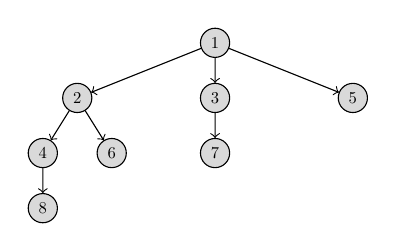
\begin{tikzpicture}[->,scale=.7,every node/.style = {scale=.6,draw,shape=circle, align=center, fill=gray!30}, level/.style={sibling distance=2.5cm/#1,level distance=1.0cm}]]
   \node[] {1}
   	   child[] { node {2} 
	   	   child {node {4}
		  	child {node {8}} 
		   }
		   child {node {6} }
	   }
   child[] { node {3}
   	   child { node {7} }
	   }
   child[] { node {5}
	}
 ;
\end{tikzpicture}
\caption{A binomial tree with nodes labeled by their positions}
\label{fig:beta}
\end{figure}

\subsubsection{Binomial trees over positive integers}

Let $k\in \mathbb{N}$ and $I=\{1,\dots,2^k\}$. 
A directed binomial tree $B^k=(V_{B^k},A_{B^k})$ with arcs oriented towards the leaves has a regular structure that allows to define a systematic numbering of nodes so that a node number determines unambiguously a position in $B^k$.
That is, we need an applicable bijective function $\beta:V_{B^k}\to I$.
A suitable bijection $\beta$ assigns values from $I$ to nodes increasingly with decreasing outgoing degree.
If there is an ambiguity, a node whose parent has a lower number is assigned a lower number.
This function is defined recursively as
\begin{equation*}
\label{eq:beta}
\beta(v)=\begin{cases}
1,\text{ if } v \text{ is the root of } B^k,\\
\beta(u) + 2^{k-deg^+(v)-1}, (u,v)\in A_{B^k},\text{ otherwise}.
\end{cases}
\end{equation*}
Nodes in Fig. \ref{fig:beta} are labeled with their $\beta$-values.
Pairs of integers that are assigned to adjacent nodes in a binomial tree are defined by relation
\begin{equation*}
\label{eq:betarel}
R=\{(i,j)\in\mathbb{N}\times\mathbb{N}:j=i+2^k,k\geq\log i,k\in \mathbb{Z}\}.
\end{equation*}

We further define the function $\pi':\mathbb{N}\to\mathbb{Z}_+$ that for a given integer $i$ associated with node $v$
determines $\beta$-value of parent of $v$: 
\begin{align*}
\label{eq:piprime}
\pi'(1)&=0,& \\
\pi'(j)&=j-2^{\lceil\log j\rceil -1}, &j > 1.
\end{align*}
Using functions $\alpha$, $\beta$, $\pi'$ and the relation $R$, we introduce the notion of binomial trees over positive integers.
\begin{definition}
A pair $(I,X)$ where $I=\{1,\dots,2^k\}$, $k\in\mathbb{Z}_+$, $(\alpha(u),\beta(u))=(\alpha(v),\beta(v))\Leftrightarrow u=v$ and
$X=\{(i,j)\in R, i,j\in I\}$ is an \emph{integer binomial tree of order $k$}. 

$(I,X)$, where $I\subseteq\{1,\dots,2^k\}, k\in \mathbb{Z}_+,\pi(j)\in I$ for all $j\in I\setminus\{1\}$ and
$X=\{(i,j)\in R, i,j\in I\}$ is an \emph{integer binomial tree of order $k$ pruned at $\{1,\dots,2^k\}\setminus I$}.
\end{definition}
We now develop a method for modelling Problem \ref{prob:min} whose main principle is finding a partition of $G$ into pruned binomial trees.
For any integer $i$, let $I_i=\{2^{i-1}+1,\dots,2^i\}$.
%\begin{problem}
%\label{prob:dec}
%Given $G=(V,E)$, $S\subseteq V$ and $t\in \mathbb{N}$, is there a sequence $S=V_0\subseteq\dots\subseteq V_t=V$ 
%and a mapping $\pi:V\setminus S\to V$, such that for each $v\in V\setminus S:\{v,\pi(v)\}\in E$ and for each  $u,v\in V_i\setminus V_{i-1}: \pi(u)\neq \pi(v)\Leftrightarrow u\neq v$?
%\end{problem}
%For a delay $t$, at most $s\cdot 2^t$ nodes can be informed within $t$ steps. 
%Therefore, we assume $n\leq 2^ks.
%This can be achieved when the broadcast forest $T$ consists of binomial trees $B^t$ of order $t$ rooted at sources $s\in S$.
%Hence, if there is a partition of $G$ into $s$ pruned binomial trees of order at most $t$ rooted at sources, then $(G,S,t)$ is a YES instance of Problem \ref{prob:dec}.
%Finding a partition of $G$ into $s$ pruned binomial trees can be equivalently formulated as finding a partition of $G''$ into $s$ (complete) binomial trees, 
%where $G''$ is constructed from $G$ as follows:
%Let $\alpha\coloneqq s\cdot 2^k-|V|$, and let $K_\alpha=(V_\alpha,E_\alpha)$ be a complete graph on $\alpha$ nodes.
%Each node in $K_\alpha$ is connected to every node $v\in V$ in the original graph $G$.
%Thus, $G''=(V'',E'')$ with $V''=V\cup V_\alpha$ and $E''=E\cup E_\alpha\cup \{\{u,v\}: u\in V \wedge v\in V_\alpha\}$.
%The set of arcs $A''$ is constructed by creating two arcs of opposite orientation for each edge, but arcs with orientation from $V_\alpha$ to $V$ are excluded. 
%Formally, $A''=A\cup\{(u,v),(v,u): \{u,v\}\in E_\alpha\}\cup\{(u,v):u\in V \wedge v\in V_\alpha\}$.

%\begin{observation}\label{obs:deg}
%For each $i\in\{1,\dots,t\}$, the set $\{v\in V^t: 1\leq\beta(v)\leq2^i\}\setminus\{v\in V^t:1\leq\beta(v)\leq2^{i-1}\}$ contains nodes with out-degree $t-i$.
%\end{observation}
%\begin{observation}\label{obs:childdeg}
%Children of $v\in V^t$ with $\text{deg}^+(v)=\ell$ have out-degree $0,\dots,\ell-1$.
%\end{observation}
\begin{observation}\label{obs:eqbetalevel}
$\pi'$ is injective.
%For $i_1,i_2\in I_i$, $\pi'(i_1)=\pi'(i_2)\Leftrightarrow i_1=i_2$.
\end{observation}
\begin{proof}
We notice that $\lceil\log (2^{i-1}+1)\rceil=\dots =\lceil\log 2^i\rceil$, and thus $\pi'(2^{i-1}+1),\dots,\pi'(2^i)$ are pairwise different.\qed 
\end{proof}

\begin{proposition}\label{lem:probeq}
A graph $G=(V,E)$ and $S\subseteq V$ has $\tau(G,S)\leq k$ iff it is possible to assign integers to nodes
such that they form $m$ (pruned) integer binomial trees of order $k$ or smaller rooted at sources.
\end{proposition}
\begin{proof}
Assume nodes in $V$ can be labeled by integers from $I=\{1,\dots,2^k\}$ so that they form (pruned) integer integer binomial trees $B_\ell$ of order at most $k$, $1\leq\ell\leq m$.
For $r\in V_{B_\ell}$ with $\alpha(r)=r$ and $\beta(r)=1$, by Obs. \ref{obs:btspread}, $\tau(B_\ell,\{r\})\leq k$.
The sequence of node sets $V_0,\dots,V_k$ is constructed by setting $V_0=\{v\in V:\beta(v)=1\}$, and $V_{i}=V_{i-1}\cup\{v\in V: \beta(v)\in I_i\}$.
Moreover, $\pi(v)=u\Leftrightarrow \alpha(v)=\alpha(u)~\&~\pi'(\beta(v))=\beta(u)$.
Also, $\pi(u)=\pi(v)\Leftrightarrow u=v$ follows from Obs. \ref{obs:eqbetalevel}, because nodes in $V_i$ have $\beta$ values in $I_i$.

Conversely, suppose there is a sequence of subsets and a function $\pi$ in $G$ with the desired properties.
Nodes are associated with integers from $I$ assigned according to the following steps:
\begin{enumerate}
\item $\beta(s)=1$ for all $s\in V_0$,
\item For $v\in V_i$, set $\beta(v)=j$ such that $j\in I_i$ and $(\pi'(\beta(v)),j)\in R, 1\leq i\leq k$.  
\end{enumerate}
\qed
\end{proof}
\subsubsection{The formulation}
Consider a graph $G'=(V',E')$ constructed  by adding a universal node $v_0$ to $G$. 
The set of nodes and edges is then $V'=V\cup \{v_0\}$ and $E'=E\cup\{\{v_0,v\}:v\in V\}$.
Apart from $z$-variables introduced in model \eqref{mod:basic}, the ILP formulation based on partition into binomial trees uses 
$$
y_{is}^v=\begin{cases}
1, \text{ if } \beta(v)=i \text{ and } \alpha(v)=s,\\ 
0, \text{ otherwise},\\
\end{cases}
$$
where $v\in V'$, $i\in I$, $s\in S$ and $0\leq j\leq \bar{t}$. 
With the definition of $G'$ above, it is straightforward to specify constraints that enforce desired values for $y$-variables.
Whenever $y_{is}^{v_0}=1$, it indicates that the binomial tree rooted at $s$ is pruned at node with position $i$.
%An obvious weakness of this approach is  that the number of nodes increases to $|V''|=\mathcal{O}(ns)$, and the dimension of variables is thus $\mathcal{O}(n^2s^2)$.
%However, once a suitable partition is found, the arcs of binomial trees contained in $K_\alpha$ can be diversely shuffled while preserving the layour of binomial trees in $G$.
%Instead of adding the entire complete graph $K_\alpha$, a single node $v_0$ with a loop $(v_0,v_0)$ is connected as an apex to the original $G$.
%Let us denote this multigraph as $G'=(V',E')$, where $V'=V\cup\{v_0\}$, $E'=E\cup\{\{u,v_0\}:u\in V\}\cup\{\{v_0\}\}$. 
%The arc set is then analogously defined as $A'=A\cup\{(u,v_0): u\in V\}\cup\{(v_0,v_0)\}$.
%The requirement for partition into binomial trees has to be adjusted accordingly.
%The subtrees contained in $G$ remain unchanged, every arc $(u,v)\in A^k_i, i=1,\dots,s$ in $G''$ with $u\in V$ and $v\in V_\alpha$ becomes $(u,v_0)$ in $G'$,
%and every $(u,v)\in A_\alpha$ becomes $(v_0,v_0)$.
%So, $v_0$ acts as a universal node that can substitute several nodes in each binomial tree.
Let us define the set $C(i)$ of $\beta$-positions of children (direct descendants) of node $v$ with $\beta(v)=i$ in a binomial tree of order $k$:
\begin{equation}
\label{eq:c1}
C(i)=\{2^j+i:j=\lceil\log_2 i\rceil,\dots,k-1\}.
\end{equation}
The formulation based on binomial trees is the following:
\begin{subequations}\label{mod:partition}
\begin{align}
\notag &\min\sum\limits_{j=0}^{\bar{t}}z_j,\\
\notag \text{s. t. } \\
\label{mod:part:nodeBelongs} \sum\limits_{i\in I}\sum\limits_{s\in S}y^v_{is} & = 1 & v\in V,\\
\label{mod:part:treeHasIJ} \sum\limits_{v\in V'}y^v_{is} & = 1 & i\in I,s\in S,\\
\label{mod:part:source1} y_{1s}^s & = 1  & s\in S,\\
%\label{mod:part:noReturn} y^u_{ij}+y^v_{lj} &\leq 1 & i\in I,l\in C(i), j\in J, u\in V_\alpha,v\in V,\\
%\label{mod:part:followArcs} y^u_{is}+y^v_{\ell s} &\leq 1 & i\in I,\ell\in C(i), s\in S, u,v\in V',(u,v)\not\in A',\\
%\label{mod:part:followArcsA} y^u_{is}+y^v_{\ell s} &\leq 1 & i\in I,\ell\in C(i), s\in S, u,v\in V,\{u,v\}\not\in E,\\
%\label{mod:part:followArcsB} y^{v_0}_{is}+y^v_{\ell s} &\leq 1 & i\in I,\ell\in C(i), s\in S, v\in V,\\
%\label{mod:part:followArcsA}y^{v_0}_{is}+y^u_{i s} + \sum\limits_{v\in V\setminus N(u)}y^v_{\ell s}&\leq 1 & u\in V,i\in I,\ell\in C(i), s\in S,  \\
%\label{mod:part:followArcsB}y^{v_0}_{is}+y^u_{\ell s} + \sum\limits_{v\in V\setminus N(u)}y^v_{i s}&\leq 1 & u\in V,i\in I,\ell\in C(i), s\in S,\\ 
\label{mod:part:followArcsA}\sum\limits_{v\in \bar{N}(u)}y^v_{\ell s}&\leq \sum\limits_{v\in N(\bar{N}(u))}y_{is}^{v} & u\in V,i\in I,\ell\in C(i), s\in S,  \\
\label{mod:part:followArcsB}\sum\limits_{v\in \bar{N}(\bar{N}(u))}y^v_{\ell s}&\leq \sum\limits_{v\in N(u)} y_{is}^{v} & u\in V,i\in I,\ell\in C(i), s\in S,\\ 
\label{mod:part:yzrel}\sum\limits_{v\in V}y^v_{is} & \leq z_{\lceil\log i\rceil} & i\in I,s\in S,\\
\label{mod:part:dim}&&y \in \{0,1\}^{I\times S\times V'}, z\in \{0,1\}^{\bar{t}}.
\end{align}~
\end{subequations}

%As the model represents the decision problem, it suffices to find any feasible solution, and no objective function is needed.
The interpretation of constraints \eqref{mod:part:nodeBelongs} is that every node in the original graph $G$ belongs to exactly one binomial tree.
Note that these constraints are quantified only over $V$ and not over $V'$.
In this way it is achieved that $v_0$ can be regarded as a part of several binomial trees.
By \eqref{mod:part:treeHasIJ} is ensured that exactly one node, possibly $v_0$, is allocated to position $i$ of each binomial tree.
By the summation over $V'$ is ensured, that pruned nodes are collectively represented by $v_0$.
Next, \eqref{mod:part:source1} enforce that source nodes are always the first nodes in corresponding binomial trees, in accordance with definition \eqref{eq:beta} of the function $\beta$.
The remaining two sets of constraints guarantee that the arcs of binomial trees follow edges in $E$.
%In particular, it is enforced by \eqref{mod:part:followArcsA} that if $u$ and $v$ are not adjacent in $G$, then $v$ must not act as a child of $u$ in any binomial tree.
In particular, it is enforced by \eqref{mod:part:followArcsA} that if there is some  non-neighbor $v$ of $u$  with a label $\ell$ in a binomial tree rooted at $s$,
then there must be a neighbor of some non-neighbor of $u$ with label $i$ in the same binomial tree.
Similarly, Constraints \eqref{mod:part:followArcsB} state that if there is a node $v$ with label $\ell$ in a binomial tree rooted at $s$ in the complement of neighborhood of all non-neighbors of $u$,
there must also be a neighbor of $u$ with label $i$ in this binomial tree. 
This reflects the obvious fact that if a tree is pruned at some node, all its descendants must also be excluded from the tree.
%The definition of $A'$ also prevents arcs of the binomial trees to be oriented from $V_\alpha$ to $V$.
%In other words, once the signal leaves the original graph $G$ and enters $v_0$, it cannot return back to $G$.
Without \eqref{mod:part:followArcsA} and \eqref{mod:part:followArcsB}, it could be possible to find a feasible solution, even when no partition of $G$ into pruned binomial trees exists.
Finally, the relation \eqref{mod:part:yzrel} between $y$ and $z$ variables follows from Obs. \ref{obs:btspread}. 
It says that whenever there is a node in a position $i$, then the delay is at least $\lceil\log i\rceil$.
%Constraints \eqref{mod:part:followArcsA} and \eqref{mod:part:followArcsB} can be replaced by stronger
%\begin{subequations}
%\begin{align}
%\label{mod:part:followArcsAStrongerA}
%y^{v_0}_{is}+y^u_{i s} + \sum\limits_{v\in V\setminus N(u)}y^v_{\ell s}&\leq 1 & u\in V,i\in I,\ell\in C(i), s\in S,  \\
%\label{mod:part:followArcsAStrongerB}
%y^{v_0}_{is}+y^u_{\ell s} + \sum\limits_{v\in V\setminus N(u)}y^v_{i s}&\leq 1 & u\in V,i\in I,\ell\in C(i), s\in S. 
%\end{align}
%\end{subequations}
%
\subsubsection{Valid inequalities}
Let $W$ be a maximal independent set in $G$.
Model \eqref{mod:partition} is strengthened by 
\begin{align}
\label{mod:part:vibasic}
y^{v_0}_{is}+ \sum\limits_{v\in W}(y^v_{is}+y^v_{\ell s})&\leq 1 & i\in I,\ell\in C(i), s\in S, 
\end{align}
which exploits the fact that no pair of nodes in $W$ is adjacent, and so there must be no two nodes with adjacent $\beta$-positions.

We now generalize this idea by using the notion of graph power $G^m=(V,E^m)$ commonly defined as a graph with the same set of nodes as $G$,
and an edge between two nodes in $G^m$ is present iff there is a path of length at most $m$ between them in $G$.
For our purposes, we use a slightly modified definition of the edge set
$$E^m=\{\{u,v\}:\text{there exists a path between $u$ and $v$ in $G$ of length $m$}\}.$$
Definition \eqref{eq:c1} can be generalized to descendants of an arbitrary distance $m$ from $v$ in $B^k$:
\begin{equation}
C^{m+1}(i)=\bigcup_{j\in C^1(i)}C^m(j).
\end{equation}
For a given $m$, let $W_m$ be a maximal independent set in $G^m$.
Further strengthening of model \eqref{mod:partition} is achieved by introducing valid inequalities
\begin{align}
\label{mod:part:vigeneral}
y^{v_0}_{is}+ \sum\limits_{v\in W_m}(y^v_{is}+y^v_{\ell s})&\leq 1 & i\in I,\ell\in C^m(i), s\in S,1\leq m\leq \Delta_G-1. 
\end{align}
Clearly, inequality \eqref{mod:part:vibasic} is included in \eqref{mod:part:vigeneral} for $m=1$.
The distance between positions $i$ and $\ell=C^m(i)$ in a binomial tree is $m$.
The maximal independent set $W_m$ contains nodes such that length of any path between any two nodes is different from $m$, 
and so there must not be two nodes in $W_m$ with positions $i$ and $\ell$ at the same time.

\subsubsection{Symmetry removal}
Another improvement of this model is achieved by a symmetry removal.
If a broadcast tree is identical to a binomial tree, we notice that nodes with labels from $C(i)$, i.e., children of some node $v$ with $\beta(v)=i$, are informed in increasing time steps.
For example in $B^3$, $C(2)=\{4,6\}$ and the corresponding nodes are informed in time step 2 and 3, respectively.
If a label $\ell\in C(i)$ corresponds to a node of a binomial tree that is pruned (if $y^{v_0}_{\ell s}=1$ for some $s\in S$), 
all labels $j\in C(i)$ such that $j>\ell$ can also be pruned. 
Thus, adding 
\begin{align}
\label{mod:part:sr}
y^{v_0}_{js}&\leq y^{v_0}_{\ell s}&i\in I,j,\ell\in C(i),j<\ell, s\in S
\end{align}
to the model reduces the set of feasible solutions.

\subsubsection{Decision version}

In a similar manner as we derived the decision version \eqref{mod:basic:dec} of model \eqref{mod:basic}, it is possible to construct a decision version of the binomial tree model \eqref{mod:partition} as follows:
\begin{subequations}\label{mod:genmatch}
\begin{align}
\notag \max\sum\limits_{v\in V}&\sum\limits_{i\in I}\sum\limits_{s\in S}   y_{is}^v,\\
\notag \text{s. t. } \\
\label{mod:genmatch:nodeBelongs} \sum\limits_{i\in I}\sum\limits_{s\in S}y^v_{is} & \leq 1 & v\in V,\\
\notag\eqref{mod:part:treeHasIJ} - \eqref{mod:part:followArcsB},\\
%\label{mod:genmatch:treeHasIJ} \sum\limits_{v\in V'}y^v_{is} & = 1 & i\in I,s\in V_T,\\
%\label{mod:genmatch:source1} y_{1s}^s & = 1  & s\in V_T,\\
%\label{mod:part:noReturn} y^u_{ij}+y^v_{lj} &\leq 1 & i\in I,l\in C(i), j\in J, u\in V_\alpha,v\in V,\\
%\label{mod:part:followArcs} y^u_{is}+y^v_{\ell s} &\leq 1 & i\in I,\ell\in C(i), s\in S, u,v\in V',(u,v)\not\in A',\\
%\label{mod:part:followArcsA} y^u_{is}+y^v_{\ell s} &\leq 1 & i\in I,\ell\in C(i), s\in S, u,v\in V,\{u,v\}\not\in E,\\
%\label{mod:part:followArcsB} y^{v_0}_{is}+y^v_{\ell s} &\leq 1 & i\in I,\ell\in C(i), s\in S, v\in V,\\
%\label{mod:genmatch:followArcsA}y^{v_0}_{is}+y^u_{i s} + \sum\limits_{v\in V\setminus N(u)}y^v_{\ell s}&\leq 1 & u\in V,i\in I,\ell\in C(i), s\in V_T,  \\
%\label{mod:genmatch:followArcsB}y^{v_0}_{is}+y^u_{\ell s} + \sum\limits_{v\in V\setminus N(u)}y^v_{i s}&\leq 1 & u\in V,i\in I,\ell\in C(i), s\in V_T,\\ 
\label{mod:genmatch:dim}&&y \in \{0,1\}^{I\times S\times V'}.
\end{align}~
\end{subequations}
This model is a modification of formulation \eqref{mod:partition}, and uses the same type of variables.
The objective function is to maximize the number of nodes involved in the binomial trees.
In order to determine the minimum broadcast time, we are looking for the minimum $k$ such that each node can be assigned a label from the set $I=\{1,\dots,2^k\}$ while satisfying given constraints.
%The index set $I=\{1,\dots,2^k\}$ depends on the input parameter $k$.
The constraints \eqref{mod:genmatch:nodeBelongs} state that each node belongs to at most one binomial tree.
Compared to \eqref{mod:part:nodeBelongs}, \eqref{mod:genmatch:nodeBelongs} is an inequality, because the binomial trees do not necessarily form a partition of $G$, and so not all nodes have to be used.
The remaining constraints are taken from formulation \eqref{mod:partition}. 

The approach is then analogous to the idea indicated in Section \ref{sec:decbasic}.
Assume we are given a lower bound $\underline{t}$ and an upper bound $\bar{t}$ on the minimum broadcast time.
Initially, we define the set $I=\{1,\dots,2^{\underline{t}}\}$ and iteratively solve the model while doubling the set $I$ until the objective function attains the value $n$.
That indicates that it is the first iteration in which all nodes are assigned a label, and it can be concluded that the minimum broadcast time is $\log_2|I|$.

%An objective function is naturally lacking in the formulation of the decision problem.
%It is nevertheless straightforward to create an ILP model for the corresponding optimization problem.
%Let $z_i=1 \Leftrightarrow t=i$ be a new variable and let $\bar{t}$ be an upper bound on the delay in $(G,S)$.
%Problem \ref{prob:min} is formulated as follows:
%\begin{subequations}
%\begin{align}
%\notag &\min\sum\limits_{j=0}^{\bar{t}}z_j,\\
%\notag \text{s. t. } \\
%\notag \eqref{mod:part:nodeBelongs} - \eqref{mod:part:source1},& \eqref{mod:part:followArcsAStrongerA} - \eqref{mod:part:followArcsAStrongerB}, \eqref{mod:part:vi}, \eqref{mod:part:sr},\\
%\notag\sum\limits_{v\in V}y^v_{is} & \leq z_{\lceil\log i\rceil} & i\in I,s\in S,\\
%\notag\label{mod:part:optdim}y &\in \{0,1\}^{I\times S\times V'}, z \in \{0,1\}^{\bar{t}}.
%\end{align}~
%\end{subequations}
